
\section{Vire payload objects}\label{app:payload}

\subsection{Introduction}

As  mentioned in  appendix \ref{app:protobuf_fmt},  Vire messages  are
wrappers for \emph{payload objects}.  Each  type of payload object can
be represented  through the \emph{protobuf} mechanism.   The following
class hierarchy shows the base architecture used to define new payload
objects.

\begin{center}
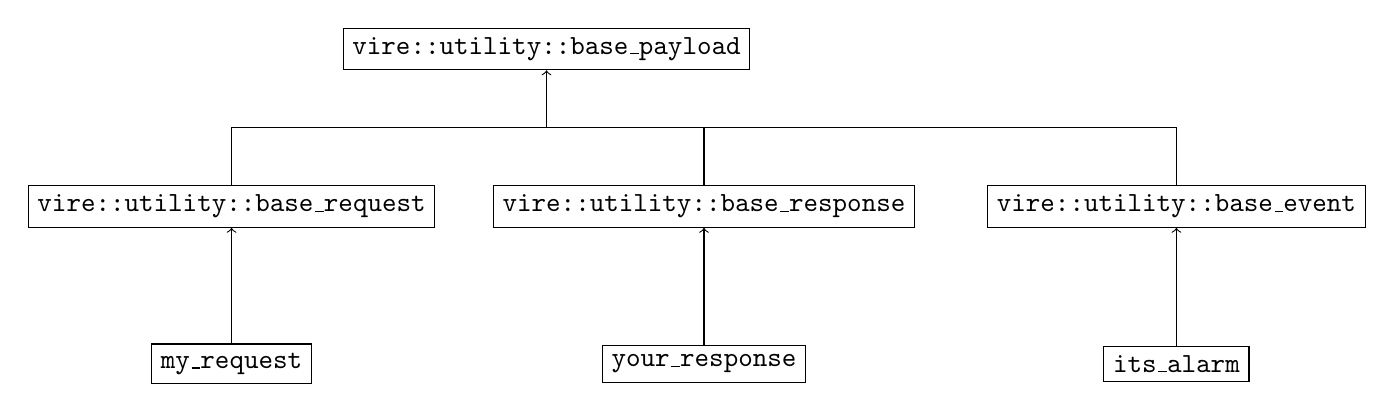
\begin{tikzpicture}
  \node (payload)  at (0,2)   [draw] {\texttt{vire::utility::base\_payload}};
  \node (request)  at (-4,0)  [draw] {\texttt{vire::utility::base\_request}};
  \node (response) at (2,0)   [draw] {\texttt{vire::utility::base\_response}};
  \node (event)    at (8,0)   [draw] {\texttt{vire::utility::base\_event}};
  \node (my)       at (-4,-2) [draw] {\texttt{my\_request}};
  \node (your)     at (2,-2)  [draw] {\texttt{your\_response}};
  \node (its)    at (8,-2)    [draw] {\texttt{its\_alarm}};

  %\draw[style=help lines] (-6,-2) grid (10,2);
  \draw (node cs:name=response,anchor=north) |- (0,1);
  \draw (node cs:name=event,anchor=north)    |- (0,1);
  \draw[->] (node cs:name=request,anchor=north)
  |- (0,1) -| (node cs:name=payload,anchor=south);
  \draw[->] (node cs:name=my,anchor=north)
  |- (-4,-1) -| (node cs:name=request,anchor=south);
  \draw[->] (node cs:name=your,anchor=north)
  |- (2,-1) -| (node cs:name=response,anchor=south);
  \draw[->] (node cs:name=its,anchor=north)
  |- (8,-1) -| (node cs:name=event,anchor=south);
\end{tikzpicture}
\end{center}


\begin{center}
\vskip 10pt
\small
\begin{tabular}{|l|l|l|}
  \hline
  \textbf{Vire C++ class} & \textbf{protobuf message type} & \textbf{protobuf definition file} \\
  \hline
  \hline
  \multicolumn{3}{|c|}{\emph{general types}} \\
  \hline
  boost::posix\_time::ptime & google.protobuf.Timestamp & google/protobuf/timestamp.proto \\
  \hline
  \hline
  \multicolumn{3}{|c|}{\emph{identifier types}} \\
  \hline
  vire::utility::base\_identifier & vire.utility.Baseidentifier & vire/utility/Baseidentifier.proto \\
  \hline
  vire::utility::instance\_identifier & vire.utility.InstanceIdentifier & vire/utility/InstanceIdentifier.proto \\
  \hline
  vire::utility::model\_identifier & vire.utility.ModelIdentifier & vire/utility/ModelIdentifier.proto \\
  \hline
  \hline
  \multicolumn{3}{|c|}{\emph{error types}} \\
  \hline
  vire::utility::base\_error & vire.utility.BaseError & vire/utility/BaseError.proto \\
  \hline
  vire::utility::invalid\_context\_error & vire.utility.InvalidContextError & vire/utility/InvalidContextError.proto \\
  \hline
  vire::utility::invalid\_setup\_id\_error & vire.utility.InvalidSetupIdError & vire/utility/InvalidSetupIdError.proto \\
  \hline
  \hline
  \multicolumn{3}{|c|}{\emph{payload types}} \\
  \hline
  vire::utility::base\_payload & vire.utility.BasePayload & vire/utility/BasePayload.proto \\
  \hline
  vire::utility::base\_request & vire.utility.BaseRequest & vire/utility/BaseRequest.proto \\
  \hline
  vire::utility::base\_response & vire.utility.BaseResponse & vire/utility/BaseResponse.proto \\
  \hline
  vire::utility::base\_event & vire.utility.BaseEvent & vire/utility/BaseEvent.proto \\
  \hline
  vire::utility::base\_alarm & vire.utility.BaseAlarm & vire/utility/BaseAlarm.proto \\
  \hline
  \hline
  \multicolumn{3}{|c|}{\emph{messenging types}} \\
  \hline
  vire::message::message\_identifier & vire.message.MessageIdentifier & vire/message/MessageIdentifier.proto \\
  \hline
  vire::message::msg\_header & vire.message.MsgHeader & vire/message/MsgHeader.proto \\
  \hline
  vire::message::msg\_body & vire.message.MsgBody & vire/message/MsgBody.proto \\
  \hline
  vire::message::message & vire.message.Message & vire/message/Message.proto \\
  \hline
\end{tabular}
\normalsize
\end{center}


\begin{center}
\vskip 10pt
\small
\begin{tabular}{|l|l|l|}
  \hline
  \multicolumn{3}{|c|}{\emph{Resource management related types}} \\
  \hline
  vire::cms::resource\_status\_record & vire.cms.ResourceStatusRecord & vire/cms/ResourceStatusRecord.proto \\
  \hline
  vire::cms::resource\_fetch\_status\_request & vire.cms.ResourceFetchStatusRequest & vire/cms/ResourceFetchStatusRequest.proto \\
  \hline
  vire::cms::resource\_fetch\_status\_success\_response & vire.cms.ResourceFetchStatusSuccessResponse & vire/cms/ResourceFetchStatusSuccessResponse.proto \\
  \hline
  vire::cms::resource\_fetch\_status\_failure\_response & vire.cms.ResourceFetchStatusFailureResponse & vire/cms/ResourceFetchStatusFailureResponse.proto \\
  \hline
  vire::cms::resource\_exec\_request & vire.cms.ResourceExecRequest & vire/cms/ResourceExecRequest.proto \\
  \hline
  vire::cms::resource\_exec\_success\_response & vire.cms.ResourceExecSuccessResponse & vire/cms/ResourceExecSuccessResponse.proto \\
  \hline
  vire::cms::resource\_exec\_failure\_response & vire.cms.ResourceExecFailureResponse & vire/cms/ResourceExecFailureResponse.proto \\
  \hline
  vire::cms::resource\_exec\_non\_blocking\_request & vire.cms.ResourceExecNonBlockingRequest & vire/cms/ResourceExecNonBlockingRequest.proto \\
  \hline
  vire::cms::resource\_exec\_non\_blocking\_ack\_response & vire.cms.ResourceExecNonBlockingAckResponse & vire/cms/ResourceExecNonBlockingAckResponse.proto \\
  \hline
  vire::cms::resource\_exec\_non\_blocking\_noack\_response & vire.cms.ResourceExecNonBlockingNoackResponse & vire/cms/ResourceExecNonBlockingNoackResponse.proto \\
  \hline
  vire::cms::resource\_exec\_non\_blocking\_success\_event & vire.cms.ResourceExecNonBlockingSuccessEvent & vire/cms/ResourceExecNonBlockingSuccessEvent.proto \\
  \hline
  vire::cms::resource\_exec\_non\_blocking\_failure\_event & vire.cms.ResourceExecNonBlockingFailureEvent & vire/cms/ResourceExecNonBlockingFailureEvent.proto \\
  \hline
  vire::cms::resource\_exec\_error & vire.cms.ResourceExecError & vire/cms/ResourceExecError.proto \\
  \hline
  vire::cms::invalid\_status\_error & vire.cms.ResourceExecError & vire/cms/ResourceExecError.proto \\
  \hline
  %% vire::cms::invalid\_credentials\_error & vire.cms.InvalidCredentialsError & vire/cms/InvalidCredentialsError.proto \\
  %% \hline
  %% vire::cms::invalid\_user\_error & vire.cms.InvalidUserError & vire/cms/InvalidUserError.proto \\
  %% \hline
  vire::cms::invalid\_resource\_error & vire.cms.InvalidUserError & vire/cms/InvalidUserError.proto \\
  \hline
  vire::cms::no\_pubsub\_resource\_error & vire.cms.NoPubsubResourceError & vire/cms/NoPubsubResourceError.proto \\
  \hline
  \hline
  \multicolumn{3}{|c|}{\emph{Resource pub/sub management types}} \\
  \hline
  vire::cms::resource\_pubsub\_subscribe\_request & vire.cms.ResourcePubsubSubscribeRequest & vire/cms/ResourcePubsubSubscribeRequest.proto \\
  \hline
  vire::cms::resource\_pubsub\_subscribe\_success\_response & vire.cms.ResourcePubsubSubscribeRSuccessResponse & vire/cms/ResourcePubsubSubscribeRSuccessResponse.proto \\
  \hline
  vire::cms::resource\_pubsub\_subscribe\_failure\_response & vire.cms.ResourcePubsubSubscribeRFailureResponse & vire/cms/ResourcePubsubSubscribeRSuccessResponse.proto \\
  \hline
  \hline
  \multicolumn{3}{|c|}{\emph{Vire/CMS server interface types}} \\
  \hline
  vire::cmsinterface::connection\_request & vire.cmsinterface.ConnectionRequest & vire/cmsinterface/ConnectionRequest.proto \\
  \hline
  vire::cmsinterface::connection\_success\_response & vire.cmsinterface.ConnectionSuccessResponse & vire/cmsinterface/ConnectionSuccessResponse.proto \\
  \hline
  vire::cmsinterface::connection\_failure\_response & vire.cmsinterface.ConnectionFailureResponse & vire/cmsinterface/ConnectionFailureResponse.proto \\
  \emph{embedded:} unknown\_resources\_error & .UnknownResourcesError &  \\
  \hline
  vire::cmsinterface::disconnection\_request & vire.cmsinterface.DisconnectionRequest & vire/cmsinterface/DisconnectionRequest.proto \\
  \hline
  vire::cmsinterface::disconnection\_success\_response & vire.cmsinterface.DisconnectionSuccessResponse & vire/cmsinterface/DisconnectionSuccessResponse.proto \\
  \hline
  %% \hline
  %% vire::cmsinterface::disconnection\_failure\_response & vire.cmsinterface.DisconnectionFailureResponse & vire/cmsinterface/DisconnectionFailureResponse.proto \\
\end{tabular}
\normalsize
\end{center}

\subsection{Basic data structures}

Any  payload object  (request, response  or event)  generally contains
some information records which are  specific to the functionalities of
the  payload  object they  belong.   These  records are  of  arbitrary
types. Of course they should be  translatable in terms of the protobuf
library.
%Of course they can be (de)serialized using JSON.
Some of these types are very  general and defined within the Vire core
API itself because they are reused by various payload objects not only
through  the Vire-CMS/LAPP  interface  but also  between  Vire clients  and
servers, independently  of the  CMS/LAPP server.  However,  the use  of the
Protocol Buffers interface makes possible  to publish the interface of
such data to the outside world, including the CMS/LAPP server in priority.

%% Other one are specific to the Vire/CMS interface and thus managed only
%% in the \texttt{Vire\_CMSInterface} API.
These  types  are considered  as  \emph{basic}.  Among them  we  find:
generic error  types, generic  identifier types,  timestamps, resource
status records\dots We propose to describe them in this section.

Once a sufficient collection of  basic data record types is available,
it  is possible  to describe  high  level payload  object types  which
aggregate attributes of such types.

Other record  types are specific to  some payload objects and  will be
never  used outside  the scope  of these  payload objects.   Such data
structures will be  explicitely declared with the  payload object they
belong to, likely as embedded types/classes.


\subsubsection{Errors}

Some  \emph{response} or  \emph{event} payload  objects may  contain a
specific  error  record  object.   A  \emph{failure  response}  or  an
\emph{exception  event}  object will  generally  embed  such an  error
record object.

Each  \emph{error record}  is represented  by an  instance of  a given
error type.   Each of  the error  types defined  in Vire  inherits the
\texttt{vire::utility::base\_error}      base       class      (figure
\ref{fig-app-payload-base_error})   which   contains   the   following
attributes:

\begin{itemize}

\item the error code: A non zero  integer which is set to 1 by default
  (indicating  a  generic  failure  case).   The  error  code  can  be
  conventionally  set to  any positive  integer value  to represent  a
  specific error case, depending on the context.

\item the error  message: an optional human  readable character string
  which documents the error as usefully as possible.

\end{itemize}

\begin{figure}[h]
\vskip 10pt
\small
\begin{Verbatim}[frame=single,xleftmargin=0.cm,label=\fbox{C++}]
struct vire::utility::base_error
{
  // Attributes:
  int         code;           // Error code (>0).
  std::string message_format; // Error message (optional).
};
\end{Verbatim}
\normalsize
\caption{The structure of a \texttt{"vire::utility::base\_error"} object
  (C++).}
\label{fig-app-payload-base_error}
\end{figure}


%% An example of JSON formatted basic error object is given in figure
%% \ref{fig-app-payload-base_error-1}.
%%
%% \begin{figure}[h]
%% \vskip 10pt
%% \small
%% \begin{Verbatim}[frame=single,xleftmargin=0.cm,label=\fbox{\texttt{JSON}}]
%% {
%%   "code" : "42",
%%   "message_format" : "Invalid AMQP server port=[2341]"
%% }
%% \end{Verbatim}
%% \normalsize
%% \caption{JSON  formatted  basic  error  object  (class
%%   \texttt{vire::utility::base\_error}.}
%% \label{fig-app-payload-base_error-1}
%% \end{figure}

Several type of generic errors are defined in Vire:


\begin{center}
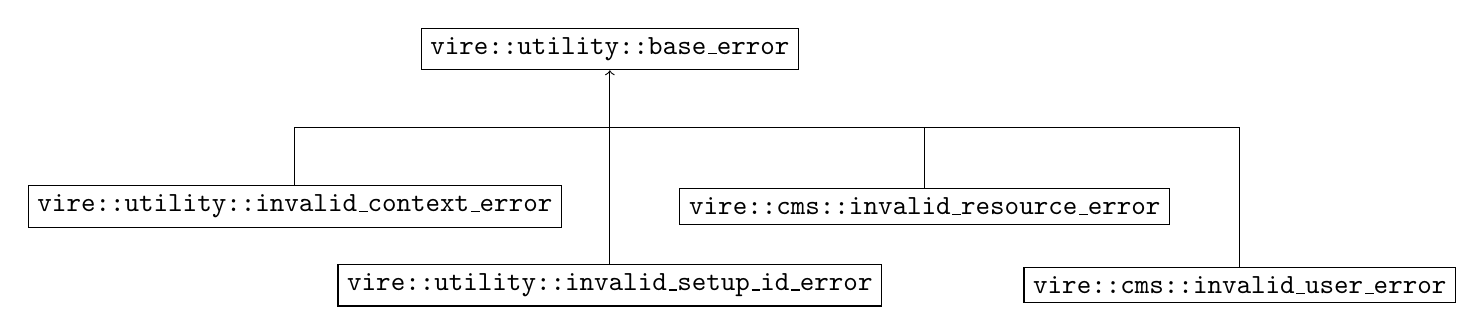
\begin{tikzpicture}
  \node (base)     at (0,2)  [draw] {\texttt{vire::utility::base\_error}};
  \node (context)  at (-4,0) [draw] {\texttt{vire::utility::invalid\_context\_error}};
  \node (setup)    at (0,-1)  [draw] {\texttt{vire::utility::invalid\_setup\_id\_error}};
  \node (resource) at (4,0)  [draw] {\texttt{vire::cms::invalid\_resource\_error}};
  \node (user)     at (8,-1)  [draw] {\texttt{vire::cms::invalid\_user\_error}};

  \draw     (node cs:name=setup,anchor=north)    |- (0,1);
  \draw     (node cs:name=resource,anchor=north) |- (0,1);
  \draw     (node cs:name=user,anchor=north)     |- (0,1);
  \draw[->] (node cs:name=context,anchor=north)
  |- (0,1) -| (node cs:name=base,anchor=south);
\end{tikzpicture}
\end{center}

\noindent
Here are a few error object types defined in Vire.  Some types belongs
to the \texttt{utility} namespace, other  ones are in the \texttt{cms}
namespace:

\begin{itemize}

\item \texttt{"vire::utility::invalid\_context\_error"} : occurs typically when
  the general context of the execution of a given resource is not adapted.\\
  It is mapped to the \texttt{"vire.utility.InvalidContextError"} protobuf record.

\item \texttt{"vire::utility::invalid\_setup\_id\_error"} : occurs in case
  of an invalid identification of the experimental setup managed
  by the Vire or CMS server.\\
  It is mapped to the \texttt{"vire.utility.InvalidSetupIdError"} protobuf record.

\item \texttt{"vire::cms::invalid\_resource\_error"} : occurs in case
  of an invalid identification of a resource.\\
  It is mapped to the  \texttt{"vire.cms.InvalidResourceError"} protobuf record.

\item \texttt{"vire::cms::invalid\_status\_error"}: occurs when an attempt
  to access a resource that has not the proper status.\\
  It is mapped to the  \texttt{"vire.cms.InvalidStatusError"} protobuf record.

\item \texttt{"vire::cms::invalid\_user\_error"} : occurs in case
  of an invalid identification of an user.\\
  It is mapped to the  \texttt{"vire.cms.InvalidUserError"} protobuf record.

\item \texttt{"vire::cms::invalid\_credentials\_error"} : occurs in case
  of user authentication error.\\
  It is mapped to the  \texttt{"vire.cms.InvalidCredentialsError"} protobuf record.

\item \texttt{"vire::cms::resource\_exec\_error"} : occurs in case
  of error at the execution of a given resource.\\
  It is mapped to the  \texttt{"vire.cms.ResourceExecError"} protobuf record.

\end{itemize}



\subsubsection{Object and type identifiers}

Vire  uses  some dedicated  classes  to  represent the  identifier  of
various objects  (or \emph{instances})  as well  as various  types (or
\emph{models})  of components.  Vire  implements  the following  class
hierarchy:

\begin{center}
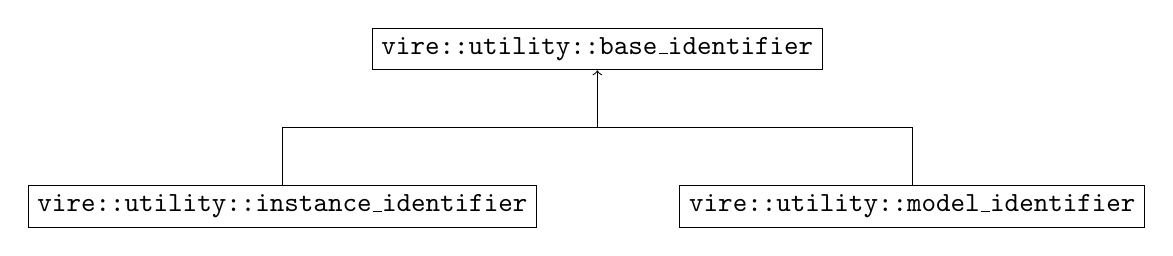
\begin{tikzpicture}
  \node (base)  at (0,2)  [draw] {\texttt{vire::utility::base\_identifier}};
  \node (instance)  at (-4,0) [draw] {\texttt{vire::utility::instance\_identifier}};
  \node (model) at (4,0)  [draw] {\texttt{vire::utility::model\_identifier}};

  \draw (node cs:name=model,anchor=north) |- (0,1);
\draw[->] (node cs:name=instance,anchor=north)
  |- (0,1) -| (node cs:name=base,anchor=south);
\end{tikzpicture}
\end{center}

The          \texttt{vire::utility::base\_identifier}          (figure
\ref{fig-app-payload-base_identifier}) class is  a pure abstract class
that cannot be instantiated. However  it contains a mandatory name and
an  optional  version description  which  are  used by  all  inherited
classes:

\begin{itemize}

\item The   \texttt{vire::utility::instance\_identifier}    concrete   class
inherits  \texttt{vire::utility::base\_identifier}  and   is  used  to
identify \underline{unique instances of objects} known by the system.

\item The  \texttt{vire::utility::model\_identifier}   concrete  class  also
inherits  \texttt{vire::utility::base\_identifier}  and   is  used  to
identify \underline{types of objects} registered in the system.

\end{itemize}

The only difference between these two classes is the validation scheme
of  the name  attribute.

\begin{figure}[h]
\vskip 10pt
\small
\begin{Verbatim}[frame=single,xleftmargin=0.cm,label=\fbox{C++}]
struct base_identifier
{
  // Attributes:
  std::string name;    // The mandatory name uniquely identifying the object or
                       // the type of object.
  std::string version; // An optional character string representing the version
                       // of the object type.
};
\end{Verbatim}
\normalsize
\caption{The structure of the \texttt{vire::utility::base\_identifier}
  class (C++).}
\label{fig-app-payload-base_identifier}
\end{figure}

%%  Figure  \ref{fig-app-payload-identifier-json}
%% shows an example of instance indentifier.
%% \begin{figure}[h]
%% \vskip 10pt
%% \small
%% \begin{Verbatim}[frame=single,xleftmargin=0.cm,label=\fbox{\texttt{JSON}}]
%% {
%%   "name" : "vire::resource::invalid_resource_error",
%%   "version" : "1.0"
%% }
%% \end{Verbatim}
%% \normalsize
%% \caption{JSON  formatted class identifier  object (class
%%   \texttt{vire::utility::model\_identifier}).   Here one  identifies a
%%   specific error type.}
%% \label{fig-app-payload-identifier-json}
%% \end{figure}


\vfill
\pagebreak
\clearpage

\subsubsection{Resource related objects}

\begin{itemize}

\item
Class \texttt{vire::cms::invalid\_resource\_error} (figure \ref{fig-app-payload-invalid_resource_error}).

\begin{center}
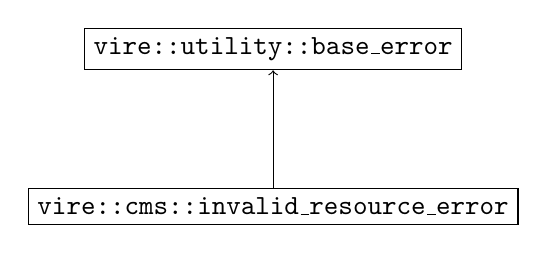
\begin{tikzpicture}
  \node (base)  at (0,2)  [draw] {\texttt{vire::utility::base\_error}};
  \node (ire)  at (0,0) [draw] {\texttt{vire::cms::invalid\_resource\_error}};
  \draw[->] (node cs:name=ire,anchor=north)
  |- (0,1) -| (node cs:name=base,anchor=south);
\end{tikzpicture}
\end{center}

\begin{figure}[h]
\vskip 10pt
\small
\begin{Verbatim}[frame=single,xleftmargin=0.cm,label=\fbox{C++}]
struct vire::cms::invalid_resource_error : public vire::utility::base_error
{
  // Attributes:
  std::string invalid_resource_path; // Invalid resource path
  std::string invalid_resource_id;   // Invalid resource internal ID (Vire server only)
};
\end{Verbatim}
\normalsize
\caption{The structure  of a invalid resource error object (C++).}
\label{fig-app-payload-invalid_resource_error}
\end{figure}

\begin{figure}[h]
\vskip 10pt
\small
\begin{Verbatim}[frame=single,xleftmargin=0.cm,label=\fbox{JSON++}]
{
  "code" : "3",
  "message_format" : "Resource path 'Atlas://Calorimeter/HV/Crate1/stop' is invalid",
  "invalid_resource_path" : "Atlas://Calorimeter/HV/Crate1/stop"
}
\end{Verbatim}
\normalsize
\caption{JSON formatted invalid resource error object.}
\label{fig-app-payload-invalid_resource_error-json}
\end{figure}


\item
Class     \texttt{vire::cms::resource\_status\_record}    (figure
\ref{fig-app-payload-resource_status_record}).

\end{itemize}

\begin{figure}[h]
\vskip 10pt
\small
\begin{Verbatim}[frame=single,xleftmargin=0.cm,label=\fbox{C++}]
struct vire::cms::resource_status_record
{
  // Attributes:
  std::string path;      // Path of the resource
  std::string timestamp; // Timestamp of the last modification
  uint16_t    flags;     // Status bits (Missing/Disabled/Pending/Error)
};
\end{Verbatim}
\normalsize
\caption{The structure  of a resource status record object (C++).}
\label{fig-app-payload-resource_status_record}
\end{figure}


\begin{figure}[h]
\vskip 10pt
\small
\begin{Verbatim}[frame=single,xleftmargin=0.cm,label=\fbox{JSON}]
{
  "path" : "SuperNEMO://Demonstrator/CMS/Coil/Control/Current/__dp_read__",
  "timestamp" : "20160612T212432.324517",
  "flags" : 2
}
\end{Verbatim}
\normalsize
\caption{JSON formatted resource status record object.}
\label{fig-app-payload-resource_status_record-json}
\end{figure}

\vfill
\pagebreak
\clearpage

\subsection{Connection of the Vire server to the CMS server}


\begin{itemize}

\item   The   \texttt{vire::cmslapp::connection\_request}   class
  (version \texttt{1.0})  represents a connection request  sent by the
  Vire server to the  CMS server through the \textcolor{blue}{service}
  channel.

\begin{center}
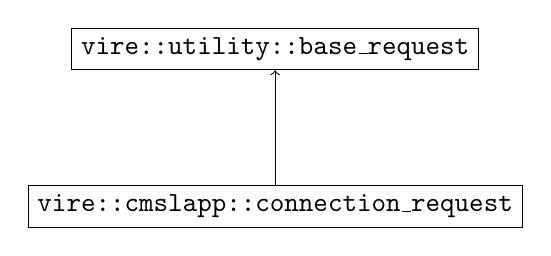
\begin{tikzpicture}
  \node (base)  at (0,2)  [draw] {\texttt{vire::utility::base\_request}};
  \node (cr)  at (0,0) [draw] {\texttt{vire::cmslapp::connection\_request}};
  \draw[->] (node cs:name=cr,anchor=north)
  |- (0,1) -| (node cs:name=base,anchor=south);
\end{tikzpicture}
\end{center}

\noindent Class registration:
\begin{itemize}
\item name: \texttt{"vire::cmslapp::connection\_request"}
\item version: "1.0"
\end{itemize}

\begin{figure}[h]
\vskip 10pt
\small
\begin{Verbatim}[frame=single,xleftmargin=0.cm,label=\fbox{C++}]
struct vire::cmslapp::connection_request : public vire::utility::base_request
{
  // Attributes:
  vire::utility::instance_identifier  setup_id; // Identifier of the experimental setup
  std::vector<std::string> requested_resources; // The list of requested resources
                                                // addressed by path
};
\end{Verbatim}
\normalsize
\caption{The structure of the connection  request object to be emitted
  by the Vire server to the CMS server (C++).}
\label{fig-app-payload-connection_request}
\end{figure}

\begin{figure}[h]
\vskip 10pt
\small
\begin{Verbatim}[frame=single,xleftmargin=0.cm,label=\fbox{JSON}]
{
  "setup_id" : {
    "name" : "snemo",
    "version" : "1.0.2"
  },
  "requested_resources" : [
    "SuperNEMO://Demonstrator/CMS/Coil/PS/Control/Current/__dp_read__",
    "SuperNEMO://Demonstrator/CMS/Coil/PS/Control/Current/__dp_write__",
    ...
    "SuperNEMO://Demonstrator/CMS/Acquisition/start",
    "SuperNEMO://Demonstrator/CMS/Acquisition/stop"
  ]
}
\end{Verbatim}
\normalsize
\caption{A JSON formatted  connection request object sent  by the Vire
  server to the CMS server (C++).}
\label{fig-app-payload-connection_request-json}
\end{figure}


\item  The  \texttt{vire::cmslapp::connection\_success\_response}
  class represents  the response sent back  to the Vire server  by the
  CMS server through the  \textcolor{blue}{service} channel in case of
  success.

\begin{center}
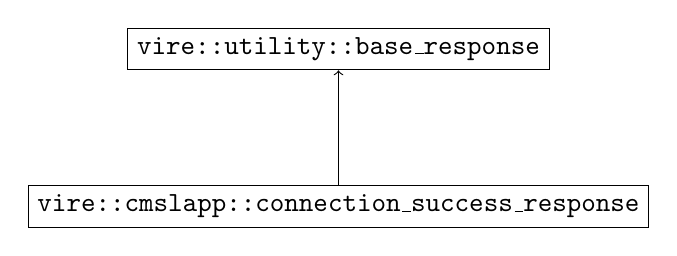
\begin{tikzpicture}
  \node (base)  at (0,2)  [draw] {\texttt{vire::utility::base\_response}};
  \node (csr)  at (0,0) [draw] {\texttt{vire::cmslapp::connection\_success\_response}};
  \draw[->] (node cs:name=csr,anchor=north)
  |- (0,1) -| (node cs:name=base,anchor=south);
\end{tikzpicture}
\end{center}

\noindent Class registration:
\begin{itemize}
\item name: \texttt{"vire::cmslapp::connection\_success\_response"}
\item version: "1.0"
\end{itemize}

\begin{figure}[h]
\vskip 10pt
\small
\begin{Verbatim}[frame=single,xleftmargin=0.cm,label=\fbox{C++}]
struct connection_success_response
  : public vire::utility::base_response
{
  typedef vire::resource::resource_status_record resource_status_record; // Type alias

  // Attributes:
  std::vector<resource_status_record> resources_snapshot; // Requested resources snapshot
};
\end{Verbatim}
\normalsize
\caption{The structure  of the connection success  response emitted by
  the CMS server to the Vire server (C++).}
\label{fig-app-payload-connection_success_response}
\end{figure}



\begin{figure}[h]
\vskip 10pt
\small
\begin{Verbatim}[frame=single,xleftmargin=0.cm,label=\fbox{\texttt{JSON}}]
{
  "resources_snapshot"  : [
    {
      "path" : "SuperNEMO://Demonstrator/CMS/Coil/PS/Control/Current/__dp_read__",
      "timestamp" : "20160612T212432.324517",
      "flags" : "0000"
    },
    {
      "path" : "SuperNEMO://Demonstrator/CMS/Coil/PS/Control/Current/__dp_write__",
      "timestamp" : "20160612T212432.328732",
      "flags" : "0000"
    },
    ...
    {
      "path" : "SuperNEMO://Demonstrator/CMS/Acquisition/start",
      "timestamp" : "20160612T212432.371671",
      "flags" : "0000"
    },
    {
      "path" : "SuperNEMO://Demonstrator/CMS/Acquisition/stop",
      "timestamp" : "20160612T212432.373624",
      "flags" : "0100"
    }
  ]
}
\end{Verbatim}
\normalsize
\caption[JSON formatted  connection success response]  {JSON formatted
  connection        success        response       object        (class
  \texttt{vire::cmslapp::connection\_success\_response}.}
\label{fig-app-payload-connection_success_response-json}
\end{figure}


\item
The  \texttt{vire::cmslapp::connection\_failure\_response}  class
represents the response sent back to the Vire server by the CMS server
through the \textcolor{blue}{service} channel in case of failure.

\begin{center}
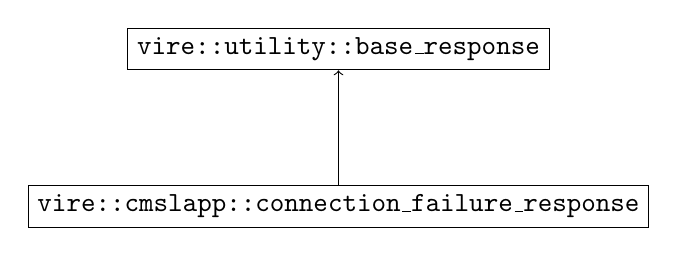
\begin{tikzpicture}
  \node (base)  at (0,2)  [draw] {\texttt{vire::utility::base\_response}};
  \node (cfr)  at (0,0) [draw] {\texttt{vire::cmslapp::connection\_failure\_response}};
  \draw[->] (node cs:name=cfr,anchor=north)
  |- (0,1) -| (node cs:name=base,anchor=south);
\end{tikzpicture}
\end{center}

\begin{figure}[h]
\vskip 10pt
\small
\begin{Verbatim}[frame=single,xleftmargin=0.cm,label=\fbox{C++}]
struct connection_failure_response
  : public vire::utility::base_response
{
  // Nested type alias:
  typedef vire::utility::model_identifier error_identifier;

  // Nested error type aliases:
  typedef vire::utility::invalid_context_error invalid_context_error;
  typedef vire::utility::invalid_setup_id_error invalid_setup_id_error;

  // Nested error type:
  struct unknown_resources_error : public vire::utility::base_error {
    std::vector<std::string> unknown_paths; // List of unknown resources' paths
  };

  // Attributes:
  error_identifier error_id; // Error type identifier
  XXX_error        error;    // Embedded error record of one of the nested error type above
};
\end{Verbatim}
\normalsize
\caption{The structure  of the  connection failure response emitted
  by the CMS server to the Vire server (C++).}
\label{fig-app-payload-connection_failure_response}
\end{figure}


\end{itemize}

% \texttt{vire::cmsserver::disconnection\_request} (version \texttt{1.0})

\vfill
\pagebreak
\clearpage


\subsection{Disconnection of the Vire server from the CMS server}

\begin{itemize}

\item  The  \texttt{vire::cmslapp::disconnection\_request}  class
  represents a  disconnection request sent  by the Vire server  to the
  CMS server through the \textcolor{blue}{service} channel.

\begin{center}
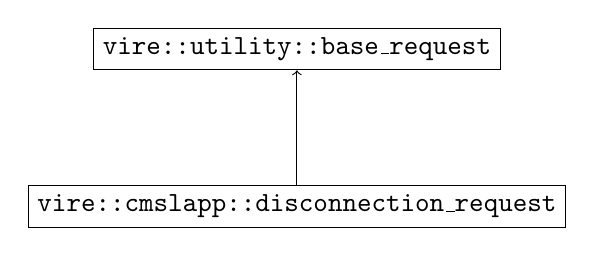
\begin{tikzpicture}
  \node (base)  at (0,2)  [draw] {\texttt{vire::utility::base\_request}};
  \node (cr)  at (0,0) [draw] {\texttt{vire::cmslapp::disconnection\_request}};
  \draw[->] (node cs:name=cr,anchor=north)
  |- (0,1) -| (node cs:name=base,anchor=south);
\end{tikzpicture}
\end{center}

\noindent Class registration:
\begin{itemize}
\item name: \texttt{"vire::cmslapp::disconnection\_request"}
\item version: "1.0"
\end{itemize}

\begin{figure}[h]
\vskip 10pt
\small
\begin{Verbatim}[frame=single,xleftmargin=0.cm,label=\fbox{C++}]
struct disconnection_request : public vire::utility::base_request {
};
\end{Verbatim}
\normalsize
\caption{The structure of the disconnection  request object to be emitted
  by the Vire server to the CMS server (C++).}
\label{fig-app-payload-disconnection_request}
\end{figure}

%% \begin{figure}[h]
%% \vskip 10pt
%% \small
%% \begin{Verbatim}[frame=single,xleftmargin=0.cm,label=\fbox{C++}]
%% {
%% }
%% \end{Verbatim}
%% \normalsize
%% \caption{A JSON formatted  connection request object sent  by the Vire
%%   server to the CMS server (C++).}
%% \label{fig-app-payload-connection_request-json}
%% \end{figure}


\item  The  \texttt{vire::cmslapp::disconnection\_success\_response}
  class represents  the response sent back  to the Vire server  by the
  CMS server through the  \textcolor{blue}{service} channel in case of
  success.

\begin{center}
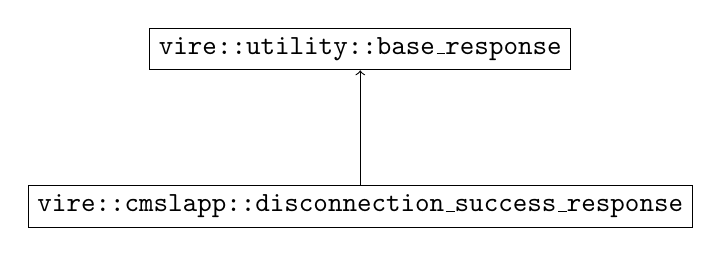
\begin{tikzpicture}
  \node (base)  at (0,2)  [draw] {\texttt{vire::utility::base\_response}};
  \node (csr)  at (0,0) [draw] {\texttt{vire::cmslapp::disconnection\_success\_response}};
  \draw[->] (node cs:name=csr,anchor=north)
  |- (0,1) -| (node cs:name=base,anchor=south);
\end{tikzpicture}
\end{center}


\noindent Class registration:
\begin{itemize}
\item name: \texttt{"vire::cmslapp::disconnection\_success\_response"}
\item version: "1.0"
\end{itemize}

\begin{figure}[h]
\vskip 10pt
\small
\begin{Verbatim}[frame=single,xleftmargin=0.cm,label=\fbox{C++}]
struct disconnection_success_response
  : public vire::utility::base_response
{
};
\end{Verbatim}
\normalsize
\caption{The structure  of the disconnection success  response emitted by
  the CMS server to the Vire server (C++).}
\label{fig-app-payload-disconnection_success_response}
\end{figure}


\end{itemize}


\vfill
\pagebreak
\clearpage

\subsection{Resource related payload objects}

\subsubsection{Resource Pub/Sub service}

\begin{itemize}

\item  The \texttt{vire::resource::resource\_pubsub\_request} object is responsible of
  demanding the activation/deactivation of the Pub/Sub service associated to a given
  resource (fig. \ref{fig-app-payload-resource_pubsub_request}).

\begin{figure}[h]
\vskip 10pt
\small
\begin{Verbatim}[frame=single,xleftmargin=0.cm,label=\fbox{C++}]
struct resource_pubsub_request
  : public vire::utility::base_request
{
  // Attributes:
  std::string path;      // The resource path.
  bool        subscribe; // Pub/Sub service (un)subscribe flag.
};
\end{Verbatim}
\normalsize
\caption{The structure of the \texttt{vire::resource::resource\_pubsub\_request}
  class (C++).}
\label{fig-app-payload-resource_pubsub_request}
\end{figure}

\item The \texttt{vire::resource::resource\_pubsub\_success\_response}
  object encapsulate a  successfull response of the CMS  server to the
  Vire  server  concerning   the  subscription/unsubscription  of  the
  Pub/Sub     service    associated     to     a    given     resource
  (fig. \ref{fig-app-payload-resource_pubsub_success_response}).

\begin{figure}[h]
\vskip 10pt
\small
\begin{Verbatim}[frame=single,xleftmargin=0.cm,label=\fbox{C++}]
struct resource_pubsub_success_response
  : public vire::utility::base_response
{
  // Pub/Sub mechanism type alias:
  typedef vire::resource::amqp_mechanism_address amqp_mechanism_address;

  // Type alias:
  typedef vire::utility::model_identifier pubsub_mechanism_identifier;
  typedef boost::variant<
      amqp_mechanism_address
      > pubsub_address_type;

  // Attributes:
  std::string                 path;               // The resource path.
  bool                        subscribe;          // The effective (un)subscribe flag.
  pubsub_mechanism_identifier pubsub_mechanism_id; // The mechanism for accessing Pub/Sub service
  pubsub_address_type         pubsub_address;      // If activation is set, this describes the
                                                   // access to the Pub/Sub service.
};
\end{Verbatim}
\normalsize
\caption{The structure of the \texttt{vire::resource::resource\_pubsub\_success\_response}
  class (C++).}
\label{fig-app-payload-resource_pubsub_success_response}
\end{figure}

\small
\begin{Verbatim}[frame=single,xleftmargin=0.cm,label=\fbox{JSON++}]
{
  "path" : "SuperNEMO://Demonstrator/CMS/Coil/PS/Monitoring/__dp_read__",
  "subscribe" : "true",
  "pubsub_mechanism_id" : "vire::amqp",
  "pubsub_address" : {
     "server" : "snemo.amqp",
     "port" : 1234,
     "channel" : "snemo.amqp.cms.pubsub.WAqq7ERzs1",
     "binding" : "SuperNEMO://Demonstrator/CMS/Coil/PS/Monitoring/__dp_read__",
     "key" : "coil.monitoring.pubsub"
  }
}
\end{Verbatim}
\normalsize

\item    The   \texttt{vire::resource::amqp\_mechanism\_address}    object
  describes   the  access   to   Pub/Sub   service  through   RabbitMQ
  (fig. \ref{fig-app-payload-amqp_pubsub_access_type}).

\begin{figure}[h]
\vskip 10pt
\small
\begin{Verbatim}[frame=single,xleftmargin=0.cm,label=\fbox{C++}]
struct amqp_mechanism_address
{
  // Attributes:
  std::string server;  // The AMQP server
  int         port;    // The AMQP server port
  std::string channel; // The RabbitMQ Pub/Sub channel.
  std::string binding; // The binding dedicated to this Pub/Sub service.
  std::string key;     // The Pub/Sub specific key/topic.
};
\end{Verbatim}
\normalsize
\caption{The structure of the \texttt{vire::resource::amqp\_pubsub\_access\_type}
  class (C++).}
\label{fig-app-payload-amqp_pubsub_access_type}
\end{figure}


\item The \texttt{vire::resource::resource\_pubsub\_failure\_response}
  object describes a failure response  concerning a request on Pub/Sub
  service       associated       to       a       given       resource
  (fig. \ref{fig-app-payload-resource_pubsub_failure_response}).


\begin{figure}[h]
\vskip 10pt
\small
\begin{Verbatim}[frame=single,xleftmargin=0.cm,label=\fbox{C++}]
struct resource_pubsub_failure_response
  : public vire::utility::base_response
{
  // Nested type alias:
  typedef vire::utility::model_identifier error_type_identifier;

  // Nested error type aliases:
  typedef vire::utility::invalid_context_error  invalid_context_error;
  typedef vire::utility::invalid_resource_error invalid_resource_error;

  // Nested error type:
  struct no_pubsub_resource_error : public vire::utility::base_error {
    std::string path; // The path of the resource without Pub/Sub service support
  };

  typedef boost::variant<
     invalid_context_error,
     invalid_resource_error,
     no_pubsub_resource_error
     > error_type;

  // Attributes:
  error_type_identifier error_type_id; // Error type identifier.
  error_type            error;        // Embedded error record of one of
                                      // the nested error types above.
};
\end{Verbatim}
\normalsize
\caption{The structure of the \texttt{vire::resource::resource\_pubsub\_failure\_response}
  class (C++).}
\label{fig-app-payload-resource_pubsub_failure_response}
\end{figure}

\end{itemize}

\vfill
\pagebreak
\clearpage

\subsubsection{Fetching resource status}

\begin{center}
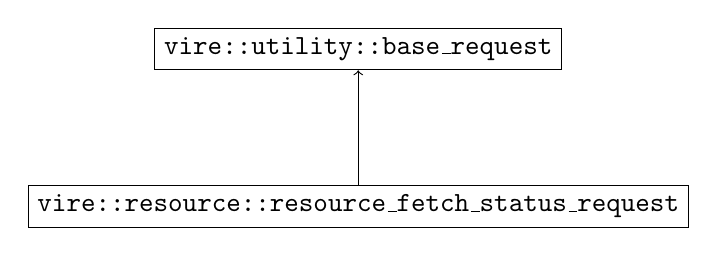
\begin{tikzpicture}
  \node (payload)  at (0,2) [draw] {\texttt{vire::utility::base\_request}};
  \node (request)  at (0,0) [draw] {\texttt{vire::resource::resource\_fetch\_status\_request}};
  \draw[->] (node cs:name=request,anchor=north)
  |- (0,1) -| (node cs:name=payload,anchor=south);
\end{tikzpicture}
\end{center}

\begin{itemize}

\item The \texttt{vire::resource::resource\_fetch\_status\_request} object
  demands to the CMS server an updated status record associated to a given resource
(fig. \ref{fig-app-payload-resource_fetch_status_request}).

\begin{figure}[h]
\vskip 10pt
\small
\begin{Verbatim}[frame=single,xleftmargin=0.cm,label=\fbox{C++}]
struct resource_fetch_status_request
  : public vire::utility::base_request
{
  // Attributes:
  std::string path; // Resource path.
};
\end{Verbatim}
\normalsize
\caption{The structure of a \texttt{vire::utility::resource\_fetch\_status\_request} object
  (C++).}
\label{fig-app-payload-resource_fetch_status_request}
\end{figure}

\item The \texttt{vire::resource::resource\_fetch\_status\_success\_response} object
  transmits the updated/current status record  associated to a given resource
(fig. \ref{fig-app-payload-resource_fetch_status_success_response}).

\begin{figure}[h]
\vskip 10pt
\small
\begin{Verbatim}[frame=single,xleftmargin=0.cm,label=\fbox{C++}]
struct resource_fetch_status_success_response
  : public vire::utility::base_response
{
  // Nested type alias:
  typedef vire::resource::resource_status_record resource_status_record;

  // Attributes:
  resource_status_record status; // The resource status record.
};
\end{Verbatim}
\normalsize
\caption{The structure of a \texttt{vire::utility::resource\_fetch\_status\_success\_response} object
  (C++).}
\label{fig-app-payload-resource_fetch_status_success_response}
\end{figure}



\item The \texttt{vire::resource::resource\_fetch\_status\_failure\_response} object
  describes a failure detected by the CMS server in response to a resource fetch status request.

\begin{figure}[h]
\vskip 10pt
\small
\begin{Verbatim}[frame=single,xleftmargin=0.cm,label=\fbox{C++}]
struct resource_fetch_status_failure_response
  : public vire::utility::base_response
{
  // Nested type alias:
  typedef vire::utility::model_identifier error_identifier;

  // Nested error type aliases:
  typedef vire::utility::invalid_context_error   invalid_context_error;
  typedef vire::resource::invalid_resource_error invalid_resource_error;

  // Attributes:
  error_identifier error_id; // Error type identifier
  XXX_error        error;    // Embedded error record of one of the nested error type above
};
\end{Verbatim}
\normalsize
\caption{The structure of a \texttt{vire::utility::resource\_fetch\_status\_failure\_response} object
  (C++).}
\label{fig-app-payload-resource_fetch_status_failure_response}
\end{figure}


\end{itemize}


\vfill
\pagebreak
\clearpage

\subsubsection{Synchronous/blocking resource execution}

\begin{center}
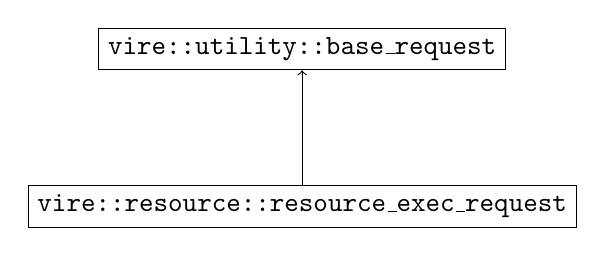
\begin{tikzpicture}
  \node (payload)  at (0,2)   [draw] {\texttt{vire::utility::base\_request}};
  \node (request)  at (0,0)  [draw] {\texttt{vire::resource::resource\_exec\_request}};
  \draw[->] (node cs:name=request,anchor=north)
  |- (0,1) -| (node cs:name=payload,anchor=south);
\end{tikzpicture}
\end{center}

\begin{itemize}

\item The \texttt{vire::resource::resource\_exec\_request} object represent a resource execution request
in blocking (synchronous) mode.


\begin{figure}[h]
\vskip 10pt
\small
\begin{Verbatim}[frame=single,xleftmargin=0.cm,label=\fbox{C++}]
struct resource_exec_request
  : public vire::utility::base_request
{
  // Type alias:
  typedef vire::resource::method_argument method_argument;

  // Attributes:
  std::string                  path;            // Resource path.
  std::vector<method_argument> input_arguments; // Embedded error record of one of
                                                // the nested error type above.
};
\end{Verbatim}
\normalsize
\caption{The structure of a \texttt{vire::utility::resource\_fetch\_status\_failure\_response} object
  (C++).}
\label{fig-app-payload-resource_fetch_status_failure_response}
\end{figure}

\item \texttt{vire::resource::resource\_exec\_success\_response}

\small
\begin{Verbatim}[frame=single,xleftmargin=0.cm,label=\fbox{C++}]
struct resource_exec_success_response
 : vire::utility::base_response
{
  // Type alias:
  typedef vire::resource::method_argument        method_argument;
  typedef vire::resource::resource_status_record resource_status_record;

  // Attributes:
  resource_status_record       status;               // Resource status
  std::string                  reception_timestamp;  // Request reception timestamp
  std::string                  completion_timestamp; // Execution completion timestamp
  std::vector<method_argument> output_arguments;     // Output arguments
};
\end{Verbatim}



\item \texttt{vire::resource::resource\_exec\_failure\_response}


\small
\begin{Verbatim}[frame=single,xleftmargin=0.cm,label=\fbox{C++}]
struct resource_exec_failure_response
 : vire::utility::base_response
{

  // Error type aliases:
  typedef vire::utility::invalid_context_error   invalid_context_error;
  typedef vire::resource::invalid_resource_error invalid_resource_error;
  typedef vire::resource::invalid_status_error   invalid_status_error;
  typedef vire::resource::resource_exec_error    resource_exec_error;

  // Type aliases:
  typedef vire::utility::model_identifier        error_type_identifier;
  typedef boost::variant<
      invalid_context_error,
      invalid_resource_error,
      invalid_status_error,
      resource_exec_error> error_type;

  // Attributes:
  error_type_identifier error_type_id; // Error type identifier
  error_type            error;        // Embedded error record

};
\end{Verbatim}

\end{itemize}


\vfill
\pagebreak
\clearpage

\subsubsection{Asynchronous/non-blocking resource execution}

\begin{center}
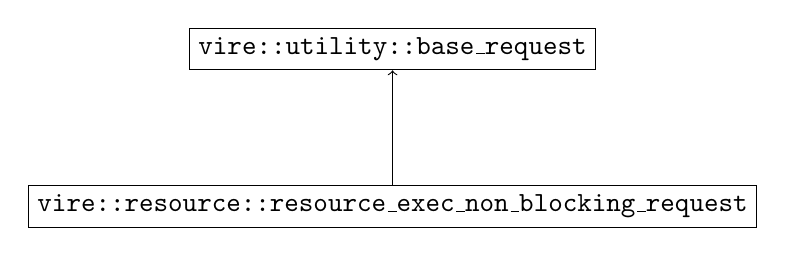
\begin{tikzpicture}
  \node (payload)  at (0,2)   [draw] {\texttt{vire::utility::base\_request}};
  \node (request_nb)  at (0,0)  [draw] {\texttt{vire::resource::resource\_exec\_non\_blocking\_request}};
  \draw[->] (node cs:name=request_nb,anchor=north)
  |- (0,1) -| (node cs:name=payload,anchor=south);
\end{tikzpicture}
\end{center}

\begin{itemize}

\item \texttt{vire::resource::resource\_exec\_non\_blocking\_request}
\small
\begin{Verbatim}[frame=single,xleftmargin=0.cm,label=\fbox{C++}]
struct resource_exec_non_blocking_request
  : public vire::utility::base_request
{
  // Type alias:
  typedef vire::resource::method_argument method_argument;

  // Attributes:
  std::string                  path;            // Resource path.
  std::vector<method_argument> input_arguments; // Embedded error record of one of
                                                // the nested error type above.

};
\end{Verbatim}

\item \texttt{vire::resource::resource\_exec\_non\_blocking\_ack\_response}


\small
\begin{Verbatim}[frame=single,xleftmargin=0.cm,label=\fbox{C++}]
struct resource_exec_non_blocking_ack_response
 : vire::utility::base_response
{
  // Type alias:
  typedef vire::resource::method_argument        method_argument;
  typedef vire::resource::resource_status_record resource_status_record;

  // Attributes:
  resource_status_record       status;
  std::string                  reception_timestamp;

};
\end{Verbatim}


\item \texttt{vire::resource::resource\_exec\_non\_blocking\_noack\_response}


\small
\begin{Verbatim}[frame=single,xleftmargin=0.cm,label=\fbox{C++}]
struct resource_exec_non_blocking_noack_response
  : vire::utility::base_response
{
  // Type alias:
  typedef vire::resource::resource_status_record resource_status_record;
  typedef vire::utility::model_identifier error_type_identifier;

  // Error type aliases:
  typedef vire::utility::invalid_context_error   invalid_context_error;
  typedef vire::resource::invalid_resource_error invalid_resource_error;
  typedef vire::resource::invalid_status_error   invalid_status_error;
  typedef vire::resource::resource_exec_error    resource_exec_error;

  // Nested error type:
  struct no_non_blocking_exec_resource_error : public vire::utility::base_error {
    std::string path; // The path of the resource without non-blocking execution support
  };

  typedef boost::variant<
     invalid_context_error,
     invalid_resource_error,
     invalid_status_error,
     no_non_blocking_exec_resource_error,
     resource_exec_error
     > error_type;

  // Attributes:
  resource_status_record status;        // Resource status.
  error_type_identifier  error_type_id; // Error type identifier.
  error_type             error;         // Embedded error record of one of
                                        // the nested error types above.

};
\end{Verbatim}
\normalsize


\item \texttt{vire::resource::resource\_exec\_non\_blocking\_success\_event}


\small
\begin{Verbatim}[frame=single,xleftmargin=0.cm,label=\fbox{C++}]
struct resource_exec_non_blocking_success\_event
  : vire::utility::base_event
{
  // Type alias:
  typedef vire::resource::method_argument        method_argument;
  typedef vire::resource::resource_status_record resource_status_record;

  // Attributes:
  resource_status_record       status;               // Resource status
  std::string                  reception_timestamp;  // Request reception timestamp
  std::string                  completion_timestamp; // Execution completion timestamp
  std::vector<method_argument> output_arguments;     // Output arguments

};
\end{Verbatim}
\normalsize

\item \texttt{vire::resource::resource\_exec\_non\_blocking\_failure\_event}


\small
\begin{Verbatim}[frame=single,xleftmargin=0.cm,label=\fbox{C++}]
struct resource_exec_non_blocking_failure\_event
  : vire::utility::base_event
{

  // Error type aliases:
  typedef vire::utility::invalid_context_error   invalid_context_error;
  typedef vire::cms::invalid_resource_error invalid_resource_error;
  typedef vire::cms::invalid_status_error   invalid_status_error;
  typedef vire::cms::resource_exec_error    resource_exec_error;

  // Type aliases:
  typedef vire::utility::model_identifier        error_type_identifier;
  typedef boost::variant<
      vire::utility::invalid_context_error,
      vire::cms::invalid_resource_error,
      vire::cms::invalid_status_error,
      vire::cms::resource_exec_error> error_type;

  // Attributes:
  error_type_identifier error_type_id; // Error type identifier
  error_type            error;        // Embedded error record

};
\end{Verbatim}
\normalsize


\end{itemize}


\vfill
\pagebreak
\clearpage

% end
